\section{Empirical evaluation}\label{sec:experiments}

We empirically evaluate the Dual Attention Transformer (abbreviated, \textit{DAT}) architecture on a range of tasks covering different domains and modalities. We begin with a synthetic relational learning benchmark to evaluate \textit{DAT}'s relational computational mechanisms in a more controlled setting. We then proceed to evaluate the proposed architecture on more complex real-world tasks, including mathematical problem-solving, image classification, and language modeling. These experiments cover multiple task paradigms and architectural variants, including: discriminative (encoder-only), sequence-to-sequence (encoder-decoder), autoregressive language modeling (decoder-only), and vision (ViT-style architecture) tasks.
% We pay particular attention to scaling with respect to model size and dataset size.
For each experiment, we fix the total number of heads, and compare different configurations of \textit{DAT} against a standard Transformer where all heads are self-attention heads. The difference in performance can be interpreted as indicating the effect of having two types of attention heads integrating sensory and relational information.
We summarize the experimental results below and defer certain experimental details to~\Cref{sec:appendix_experimental_details}.

\subsection{Sample-Efficient Relational Reasoning: Relational Games}\label{ssec:relgames}

We begin our empirical evaluation with the ``Relational Games'' benchmark for visual relational reasoning contributed by~\citet{shanahanExplicitlyRelationalNeurala}. The dataset consists of a family of binary classification tasks, each testing a model's ability to identify a particular visual relationship among a series of objects. The input is an RGB image depicting a grid of objects, and the target is a binary classification indicating whether the particular relation holds for this input. This forms a controlled synthetic setting for evaluating \textit{DAT}'s effectiveness in relational learning.

Our goal in this section is explore how the relational computational mechanisms of \textit{DAT} affect data-efficiency in relational learning---that is, how much data is necessary to learn a given task. We evaluate \textit{learning curves} by varying the size of the training set, training each model until convergence, and evaluating on a hold-out validation set. We test two configurations of \textit{DAT}: one with only relational attention heads, and one with a combination both sensory and relational heads. We include several Transformer baselines, varying the number of attention heads and the model dimension (e.g., to control for parameter count). We repeat each experimental run 5 times with different random seeds to compute approximate confidence intervals. The results are depicted in~\Cref{fig:relgames_learning_curves}.

We find that \textit{DAT} is significantly more sample-efficient, particularly at more difficult tasks. Both configurations of \textit{DAT} are consistently more sample-efficient compared to the standard Transformer. The effect is particularly dramatic on the `\texttt{match pattern}' task which is the most difficult and requires identifying a ``second-order'' relation (a relation between relations). We note that these tasks are ``purely relational'' in the sense that pairwise same/different relations between objects are a sufficient statistic for predicting the target. This suggests that relational attention is sufficient for solving the task. Indeed, the \textit{DAT} variant with only relational heads performs marginally better than the variant with a combination of both sensory and relational heads. Notably, however, the difference is only marginal, suggesting that the model is able to learn to select the computational mechanisms that are most relevant to the given task. We provide further discussion in~\Cref{ssec:appendxi_relgames}, including results comparing against previously-proposed relational architectures.


\begin{figure}
    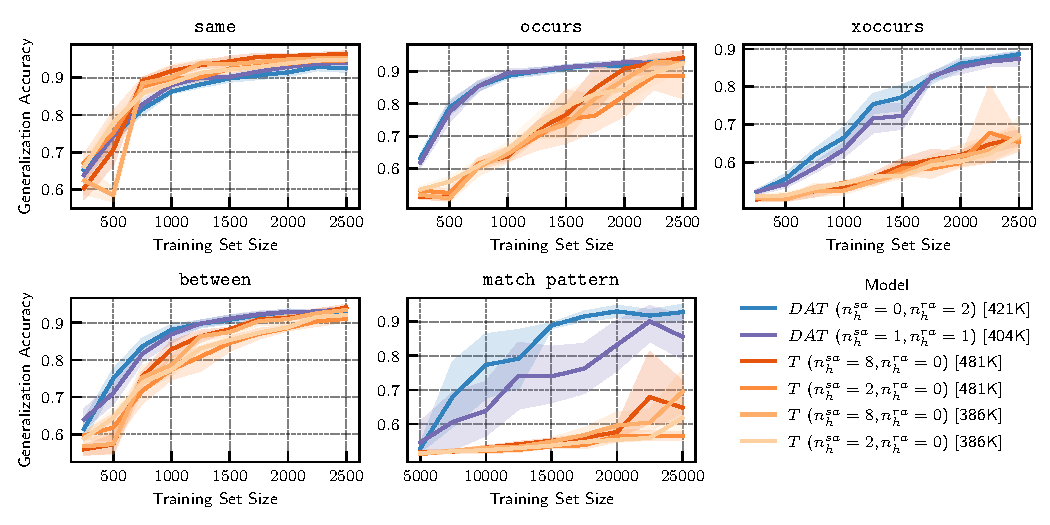
\includegraphics[width=\textwidth]{figs/experiments/relgames/relgames_learning_curves_transformer_comparison.pdf}
    \caption{\textit{DAT} is more data-efficient at relational learning compared to a Transformer. Learning curves on the relational games benchmark. Solid lines indicate the mean over 5 trials with different random seeds and the shaded regions indicate bootstrap 95\% confidence intervals.}\label{fig:relgames_learning_curves}
\end{figure}

% In this experiment, we use positional symbols as the symbol assignment mechanism since the objects can be identified through their position on the grid. We also impose symmetry on the relations in relational attention, which we find to be a useful inductive bias. Intuitively, this is because the task-relevant relations are symmetric similarity relations across different visual attributes. We provide further discussion in~\Cref{ssec:appendxi_relgames}, including results comparing against previously-proposed relational architectures.

\subsection{Relational Inductive Biases for Symbolic Reasoning in Sequence-to-Sequence tasks: Mathematical Problem Solving}\label{ssec:math}

Next, we evaluate \textit{DAT} on a set of mathematical problem-solving tasks based on the benchmark contributed by~\citet{saxtonAnalyzingMathematicalReasoning2019}. We use this as a proxy for ``symbolic reasoning''. Mathematical problem-solving is an interesting test for neural models because it requires more than statistical pattern recognition---it requires inferring laws, axioms, and symbol manipulation rules. The benchmark consists of a suite of mathematical problem-solving datasets, with each dataset consisting of a set of question-answer pairs. The tasks range across several modules or topics including solving equations, adding polynomials, expanding polynomials, differentiating functions, predicting the next term in a sequence, etc. For instance, an example of question in the `\texttt{polynomials\_\_expand}' task is ``\texttt{Expand (5*x - 3) * (2*x + 1)}'' with the target answer ``\texttt{10 * x ** 2 - x - 3}''. This is modeled as a sequence-to-sequence task with character-level encoding.

\aawarning{To add somewhere: we refer to standard attention as "sensory attention" because it attends to sensory information, whereas relational attention attends to relational information. $\nhsa$ refers to the number of standard self-attention heads (i.e., sensory attention heads).}

We compare \textit{DAT} against Transformers following an encoder-decoder architecture. The encoder processes the question, and the decoder autoregressively generates the answer while cross-attending to the encoder. We explore how performance scales with model size by varying the number of layers. In the Transformer, all attention heads are standard self-attention, $\nhsa = 8$, while in \textit{DAT} we have a combination of both types of attention heads with $\nhsa = \nhra = 4$. The \textit{DAT} models use position-relative symbols as their symbol assignment mechanism.

\Cref{fig:math_scaling} depicts model performance, measured as character-level accuracy on a hold-out test set, for \textit{DAT} and Transformers as model size varies. We find that the \textit{DAT} model outperforms the standard Transformer at all model scales across all tested tasks. This suggests that the relational computational mechanisms of \textit{DAT} are useful for the type of symbolic processing involved in solving mathematical problems.


% We compare \textit{DAT} against a Transformer using matching encoder-decoder architectures. We use 2-layer models with the total number of heads fixed to $8$ in both the encoder and the decoder. We compare an encoder-decoder Transformer with $\nhsa = 8$ against two configurations of \textit{DAT}: one with $\nhsa = \nhra = 4$ for the encoder and $\nhsa = 8, \nhra = 0$ for the decoder (config 1) and another with $\nhsa = \nhra = 4$ for both the encoder and decoder (config 2). The number of cross-attention heads is $8$ in all cases. The \textit{DAT} models use position-relative symbols as their symbol assignment mechanism.

% \begin{figure}
%     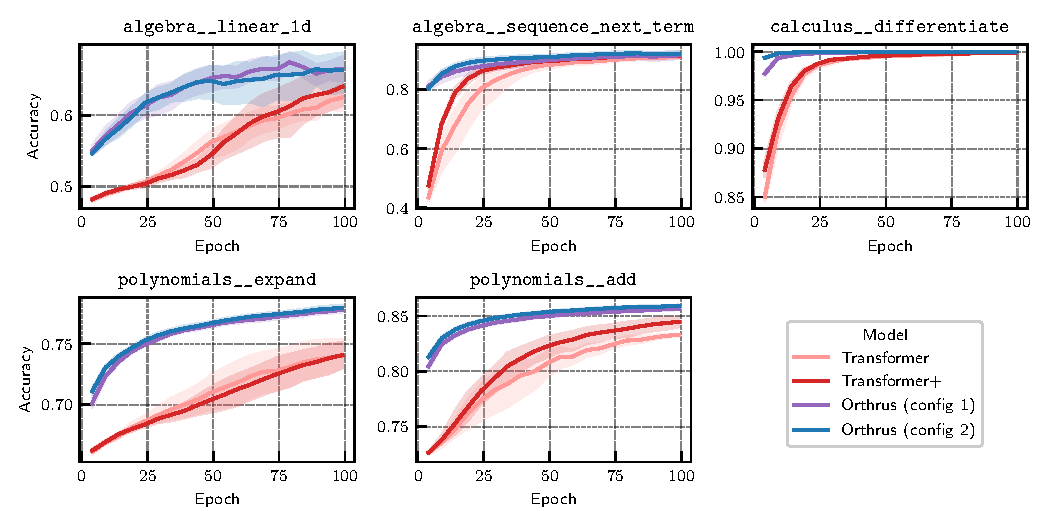
\includegraphics[width=\textwidth]{figs/experiments/math/math_training_curves_interpolation.pdf}
%     \caption{Validation accuracy over the course of training on mathematical problem-solving tasks. \textit{DAT} learns faster and reaches higher accuracy. Solid lines indicate mean over 5 trials with different random seeds, and shaded regions indicate 95\% bootstrap confidence intervals.}\label{fig:math_training_curves_interpolation}
% \end{figure}

\begin{figure}
    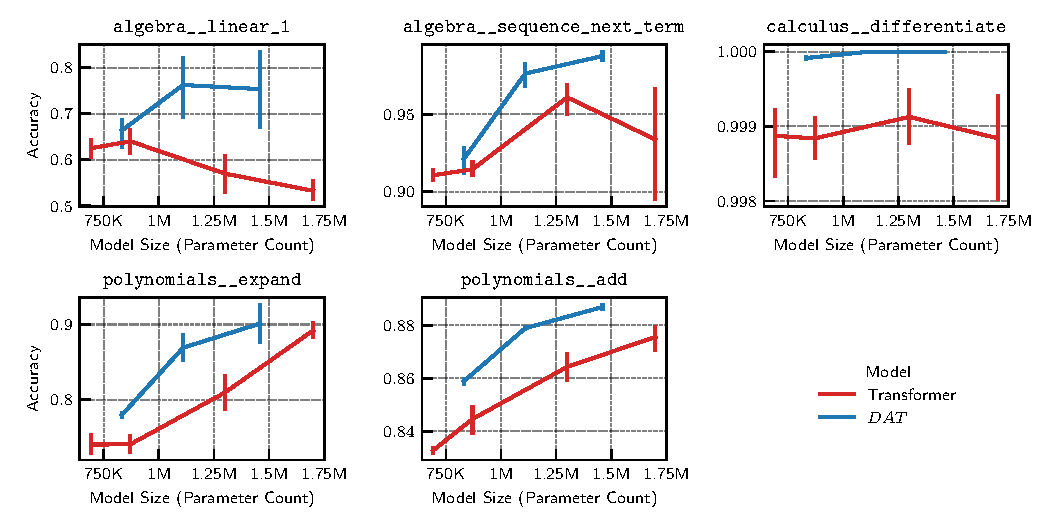
\includegraphics[width=\textwidth]{figs/experiments/math/math_accuracy_scaling.pdf}
    \caption{Average character-level accuracy on different mathematical problem-solving tasks measured at different model sizes. Error bars indicate bootstrap 95\% confidence intervals over 5 trials. \textit{DAT} outperforms a standard Transformer across model schools, suggesting that relational computational mechanisms confer benefits on sequence-to-sequence tasks that involve certain types of symbolic computation.}\label{fig:math_scaling}
\end{figure}

% \begin{table}
%     \begin{tabular}{l|l|cc}
\toprule
Task & Model &  Accuracy \\
\midrule
\multirow{7}{*}{$\texttt{algebra\_\_linear\_1d}$} & Transformer [692K] &                    62.5\% \\
                                 & $DAT$ [783K] &                    66.5\% \\
                                 & Transformer [871K] &                    64.0\% \\
                                 & $DAT$ [1.09M] &                    76.6\% \\
                                 & Transformer [1.3M] &                    64.3\% \\
                                 & $DAT$ [1.43M] &                    74.7\% \\
                                 & Transformer [1.7M] &                    50.9\% \\
\cline{1-3}
\multirow{7}{*}{$\texttt{algebra\_\_sequence\_next\_term}$} & Transformer [692K] &                    91.1\% \\
                                 & $DAT$ [783K] &                    91.6\% \\
                                 & Transformer [871K] &                    91.4\% \\
                                 & $DAT$ [1.09M] &                    97.3\% \\
                                 & Transformer [1.3M] &                    96.9\% \\
                                 & $DAT$ [1.43M] &                        -- \\
                                 & Transformer [1.7M] &                    82.6\% \\
\cline{1-3}
\multirow{7}{*}{$\texttt{calculus\_\_differentiate}$} & Transformer [692K] &                    99.9\% \\
                                 & $DAT$ [783K] &                   100.0\% \\
                                 & Transformer [871K] &                    99.9\% \\
                                 & $DAT$ [1.09M] &                        -- \\
                                 & Transformer [1.3M] &                    99.9\% \\
                                 & $DAT$ [1.43M] &                   100.0\% \\
                                 & Transformer [1.7M] &                   100.0\% \\
\cline{1-3}
\multirow{7}{*}{$\texttt{polynomials\_\_add}$} & Transformer [692K] &                    83.3\% \\
                                 & $DAT$ [783K] &                    85.6\% \\
                                 & Transformer [871K] &                    84.5\% \\
                                 & $DAT$ [1.09M] &                    87.9\% \\
                                 & Transformer [1.3M] &                    86.9\% \\
                                 & $DAT$ [1.43M] &                    88.7\% \\
                                 & Transformer [1.7M] &                    87.3\% \\
\cline{1-3}
\multirow{7}{*}{$\texttt{polynomials\_\_expand}$} & Transformer [692K] &                    74.0\% \\
                                 & $DAT$ [783K] &                    77.8\% \\
                                 & Transformer [871K] &                    74.1\% \\
                                 & $DAT$ [1.09M] &                        -- \\
                                 & Transformer [1.3M] &                        -- \\
                                 & $DAT$ [1.43M] &                    92.2\% \\
                                 & Transformer [1.7M] &                    87.2\% \\
\bottomrule
\end{tabular}

% \end{table}


% Each model is trained for 100 epochs, and accuracy on a hold-out validation set is tracked over the course of training. For each model and task, we run 5 trials with different random seeds to compute approximate confidence intervals. We find that \textit{DAT} models learn faster and reach higher accuracies compared to a standard Transformer.

\subsection{Visual Processing with Relational Inductive Biases}\label{ssec:vision}

As a general sequence model, the Transformer architecture can be applied to visual inputs by dividing an RGB image into patches that are then flattened, linearly embedded into vectors, and passed in as a sequence. Through a series of attention and MLP operations, the visual input is processed for the downstream visual task (e.g., image recognition). This architecture is referred to as a Vision Transformer (\textit{ViT}) and was first explored by~\citet{dosovitskiyImageWorth16x162020}. Although the Transformer lacks the explicit spatial inductive biases of models like convolutional networks, recent work has shown that this architecture can be effective at scale~\citep{addcitations}, suggesting that attention is a versatile computational mechanism applicable to a wide range of data modalities.

In this section, we explore how the relational computational mechanisms introduced in \textit{DAT}---namely, relational attention---impact visual processing tasks. Our hypothesis is that visual processing involves attending over both sensory and relational information. That is, when processing a local region of a visual input (e.g., a patch, object, or object part), it is useful to attend to not only the sensory features of other regions of the input, but also the visual relationships with other regions of the input. For example, this captures information about similar objects occurring in multiple places in the scene, or objects which are similar across some attributes (e.g., texture) but different across others (e.g., color).

\begin{table}
    % \begin{tabular}{@{}l|ccccccc|c@{}}
\begin{tabular}{@{}lcc|cccccc|c@{}}
    \toprule
    Model        & Param count   & \# Tokens &$\dmodel$&$\nlayers$& $\nhsa$  & $\nhra$ & $d_r$ & $n_{kv}^{h}$ & Perplexity $\downarrow$ \\ \midrule\hline
    Transformer  & 353M   & 10B       & 1024    & 24       & 16       & -        & -     & -           & 16.94     \\
    \textit{DAT} & 343M   & 10B       & 1024    & 24       & 8        & 8        & 8    & 4           & 16.26     \\
    \textit{DAT} & 343M   & 10B       & 1024    & 24       & 8        & 8        & 32    & 4           & 16.14     \\
    \textit{DAT} & 343M   & 10B       & 1024    & 24       & 8        & 8        & 64    & 4           & 16.09     \\
    % \textit{DAT} & 368M   & 10B       & 1024    & 24       & 8        & 8        & 8   & 8           & 15.97     \\\midrule
    Transformer  & 1.31B  & 10B       & 2048    & 24       & 32       & -        & -     & -           & 13.63     \\
    \textit{DAT} & 1.27B  & 10B       & 2048    & 24       & 16       & 16       & 64    & 8           & 13.44     \\
    \textit{DAT} & 1.37B  & 10B       & 2048    & 24       & 16       & 16       & 64    & -          & 13.43     \\ \bottomrule
    % Model / Param count   &$\dmodel$&$\nlayers$& $\nhsa$  & $\nhra$ & $n_r$ & $n_{kv}^{h}$ & Perplexity $\downarrow$ \\ \midrule\hline
    % Transformer - 353M   & 1024    & 24       & 16       & -        & -     & -           & 16.944     \\
    % \textit{DAT} - 343M  & 1024    & 24       & 8        & 8        & 32    & 4           & 16.258     \\
    % \textit{DAT} - 368M  & 1024    & 24       & 8        & 8        & 32    & 8           & 15.969     \\\midrule
    % Transformer - 1.31B  & 2048    & 24       & 32       & -        & -     & -           & 13.630     \\
    % \textit{DAT} - 1.27B & 2048    & 24       & 16       & 16       & 64    & 8           & 13.440     \\
    % \textit{DAT} - 1.37B & 2048    & 24       & 16       & 16       & 64    & 16          & 13.426     \\ \bottomrule
\end{tabular}%
    % }
    % & $n_s$ 
    % & -     
    % & 1024  
    % & 1024  
    % & -     
    % & 512   
    % & 2048  
    \vskip5pt
    \caption{Classification accuracy on image recognition with the CIFAR-10 and CIFAR-100 datasets. Each training configuration is repeated 10 times with different random seeds; we report the mean accuracy $\pm$ the standard error of mean. \textit{DAT} outperforms a standard Vision Transformer, suggesting that relational computational mechanisms are useful for visual processing tasks.}\label{tab:cifar_results}
\end{table}

We evaluate a \textit{ViT}-style \textit{DAT} architecture, and compare against a standard \textit{ViT} on the CIFAR image recognition benchmarks~\citep{cifar_dataset}. We train directly on CIFAR-10 and CIFAR-100, respectively, without pretraining on larger datasets. We use random cropping, MixUp~\citep{zhang2018mixup}, and CutMix~\citep{yun2019cutmix} as data augmentation techniques during training. In~\Cref{ssec:appendix_vision} we also report results using AutoAugment~\citep{cubuk2019autoaugmentlearningaugmentationpolicies}. We evaluate 8-layer models with $\dmodel = \dff = 384$. The \textit{ViT} model has $\nhsa = 12$ standard self-attention heads, while the \textit{DAT} model uses both sensory and relational heads, with an even split $\nhsa = \nhra = 6$. We use symmetric relations $\bm{r}_{ij}$ with the intuition that visual processing involves symmetric attribute-similarity relations (see~\Cref{ssec:appendix_vision} for ablations and further discussion). We use position-relative symbols as the symbol assignment mechanism.
% We give the standard Transformer an advantage in terms of parameter count by reducing the number trainable parameters in the \textit{DAT} by using Grouped Query Attention.

\Cref{tab:cifar_results} reports the classification accuracy of each model. We find that the vision \textit{DAT} architecture outperforms the standard \textit{ViT} architecture across both datasets, suggesting that the relational computational mechanisms confer benefits in visual processing.

These experiments show that relational inductive biases can be useful for image recognition. We hypothesize that relational processing is even more important in visual tasks that involve parsing complex viusal scenes through some type of \textit{reasoning} about the relationships between its constituent objects. For example, see recent work probing scene understanding in large vision-language models~\citep{johnson2017clevr,zerroug2022benchmark,zhao2024benchmarking}. We leave exploration of this to future work.

\aafatal{Decide what to do with the imagenet results. Remove for now?}

% \subsection{The Benefits of Relational Inductive Biases in Vision: Image Recognition with ImageNet}\label{ssec:imagenet}

% In the final set of experiments, we evaluate \textit{DAT} on a vision task---object classification with the ImageNet dataset~\citep{imagenet}. This further probes \textit{DAT}' ability in different modalities as a general-purpose sequence model. This section also stress tests \textit{DAT} at larger scales.

% \begin{figure}[ht]
%     \centering
%     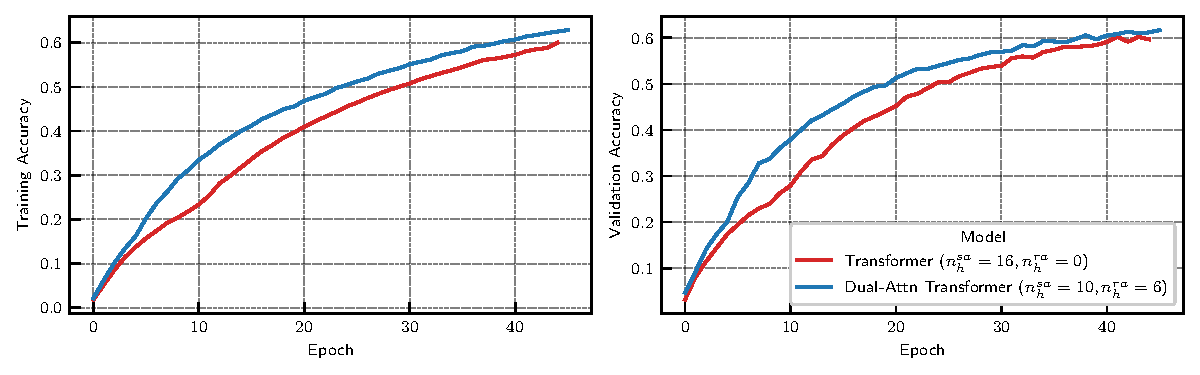
\includegraphics[width=0.9\textwidth]{figs/experiments/imagenet/imagenet_acc_curves.pdf}
%     \caption{\textit{DAT} compared to a Vision Transformer on image recognition with ImageNet. \textit{DAT} learns faster and achieves better performance.}\label{fig:vision_acc_curve}
% \end{figure}

% Here, we again use a Vision Transformer-style architecture \citep{dosovitskiyImageWorth16x162020}. ImageNet's RGB images are divided into $16 \times 16$ patches, flattened, and linearly embedded into a vector. A learnable positional embedding is added to each patch embedding. We also prepend a special classification token. The sequence of patch embeddings is then fed through an Encoder and the embedding of the class token is used to generate the final classification through a fully connected layer. We compare a Vision Transformer model with $n_h^{sa} = 16$ to an \textit{DAT} model with $n_h^{sa} = 10, n_h^{sa} = 6$. For both, we used a model dimension $\dmodel = 1024$ and $L = 24$ layers. The \textit{DAT} model uses position-relative symbols as the symbol assignment mechanism and symmetric relational attention.

% \Cref{fig:vision_acc_curve} depicts the training and validation accuracy over the course of training. We find that \textit{DAT} learns significantly faster. Averaging over epochs, \textit{DAT} has 5.0 (resp., 4.4) percentage points higher training accuracy (resp., validation accuracy) over the course of training compared to a standard Vision Transformer. At the end of training, \textit{DAT} maintains a 2.9 (resp., 1.5) percentage point advantage. This suggests that relational processing is important in processing visual scenes. This matches our intuition that parsing a visual scene requires reasoning about the visual relations between different objects or parts in the scene.

\aafatal{decide what to do with tiny stories experiments... remove? move to appendix?}

% \subsection{Improvements in Language Modeling (Tiny Stories)}\label{ssec:tiny_stories}

% In this section, we evaluate \textit{DAT} on autoregressive language modeling. Transformer language models are typically built on what is sometimes called a ``decoder-only'' architecture. The model receives a sequence of tokens as input and is trained to causally predict the next token at each position.

% We evaluate the language modeling capabilities of \textit{DAT}, as compared to standard Transformers, using the ``Tiny Stories'' dataset of~\citet{eldanTinyStoriesHowSmall2023}. The dataset consists of short stories and is intended as a benchmark for small language models. Again, for each configuration, we fix the total number of attention heads, and compare a Transformer with only standard self-attention heads to \textit{DAT} models with a mix of self-attention and relational attention heads. We compare a Transformer with $\nhsa = 8$ attention heads to two configurations of \textit{DAT}, one with $\nhsa = 6, \nhra = 2$ and another with $\nhsa = \nhra = 4$.

% \begin{figure}[ht]
%     \begin{subfigure}{0.33\textwidth}
%         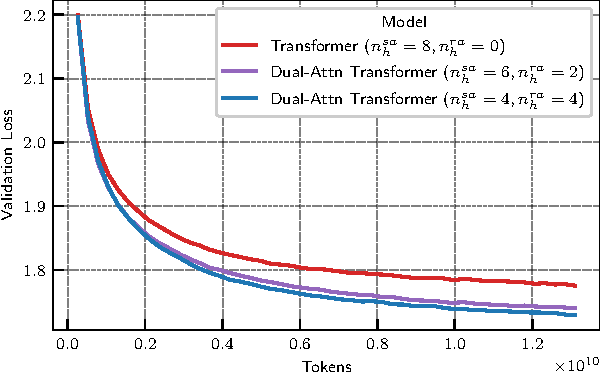
\includegraphics[width=\textwidth]{figs/experiments/tiny_stories/d64L4_symattn_asymra.pdf}
%         \caption{4 Layers}
%     \end{subfigure}
%     \begin{subfigure}{0.33\textwidth}
%         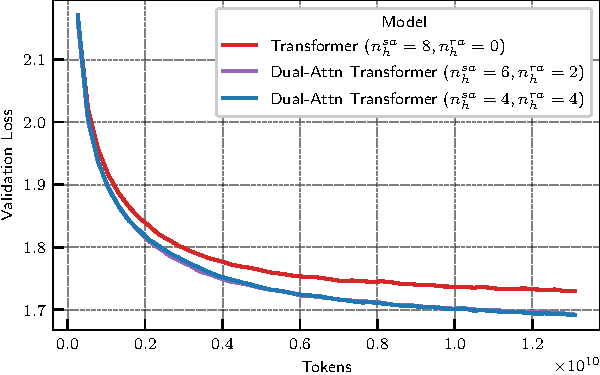
\includegraphics[width=\textwidth]{figs/experiments/tiny_stories/d64L5_symattn_asymra.pdf}
%         \caption{5 Layers}
%     \end{subfigure}
%     \begin{subfigure}{0.33\textwidth}
%         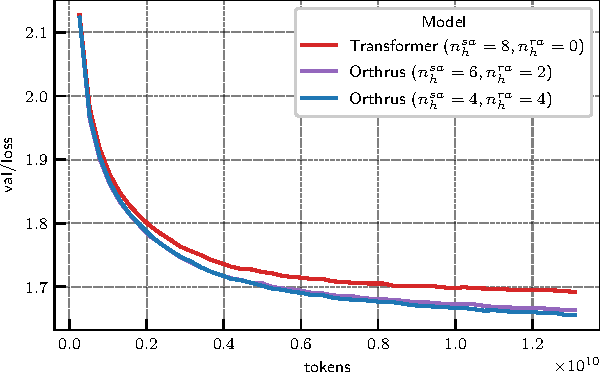
\includegraphics[width=\textwidth]{figs/experiments/tiny_stories/d64L6_symattn_asymra.pdf}
%         \caption{6 Layers}
%     \end{subfigure}
%     \caption{Validation loss curves on a language modeling task. The $x$-axis indicates the number of tokens and the $y$-axis is the validation loss. \textit{DAT} achieves a smaller validation loss for the same total number of attention heads.}\label{fig:tiny_stories_val_loss_curves}
% \end{figure}

% \Cref{fig:tiny_stories_val_loss_curves} depicts the validation loss throughout training for each model. We find that \textit{DAT} models with dual head attention achieve lower loss for the same total number of attention heads. We also varied the number of layers, and observed that the trend persists as the number of layers increases. The effect is small but consistent. The two \textit{DAT} configurations behave similarly, with perhaps a very slight advantage to $\nhsa = \nhra = 4$ (the configuration with a balanced composition of head types).

% In~\Cref{fig:tiny_stories_val_loss_curves}, the \textit{DAT} models use \textit{symbolic attention} as the symbol assignment mechanism and asymmetric relations in relational attention. We find that symbolic attention outperforms position-relative symbols on this language modeling task. In fact, with position-relative symbols, there is no discernable advantage over the Transformer. Symbolic attention may be well-suited to language due to its implementation of a learned differentiable equivalence class mapping, which can perhaps be thought of as a form of syntax. We also find that asymmetric relations in relational attention perform better than symmetric relations. This may be because the relevant relations in language modeling are asymmetric (e.g., asymmetric syntactic or grammatical relations such as noun-verb, subject-object, determiner-noun, etc.). We provide further discussion and present ablations in~\Cref{ssec:appendix_lm}.

% We conclude this section by noting that modern large language models are applied to diverse and multi-modal tasks, where different inductive biases will be useful in different contexts. While the language models explored in this section are small, an interesting avenue for future research would be to investigate whether the observed performance benefits scale up to larger models.

\subsection{Relational Inductive Biases in Language Modeling}\label{ssec:fineweb}

Language understanding involves processing and organizing relational information, such as syntactic structures, semantic roles, and contextual dependencies, to extract meaning from words and their connections within sentences. Transformers have been remarkably effective at language modeling, with neural scaling laws demonstrating that increasing model size and dataset size result in predictable improvements in performance across a range of language tasks \citep{kaplan2020scalinglawsneurallanguage}. While the standard attention mechanism of Transformers is able to capture simple positional and syntactic relations in its attention scores, this is only used to control the flow of information between tokens rather than explicitly encoding relational information in the token embeddings themselves. The relational attention mechanism of \textit{DAT} enables explicitly learning relational contextual information that is directly encoded in each token's hidden embedding.

In this section, we evaluate \textit{DAT} on causal language modeling, exploring the effects of its relational computational mechanisms in the domain of language. We use a ``decoder-only'' architecture, where the model receives a sequence of tokens as input and is trained to causally predict the next token at each position. We train on 10 billion GPT2 tokens of the FineWeb-Edu dataset~\citep{lozhkov2024fineweb-edu}, which is a curated dataset of high-quality educational text data from CommonCrawl. We train models at multiple parameter scales to study the scaling properties of \textit{DAT} on language modeling with respect to both model size and data size. Details of training and architectural hyperparameters are given in~\Cref{ssec:appendix_fineweb}, together with further discussion of the results.

\begin{figure}
    \centering
    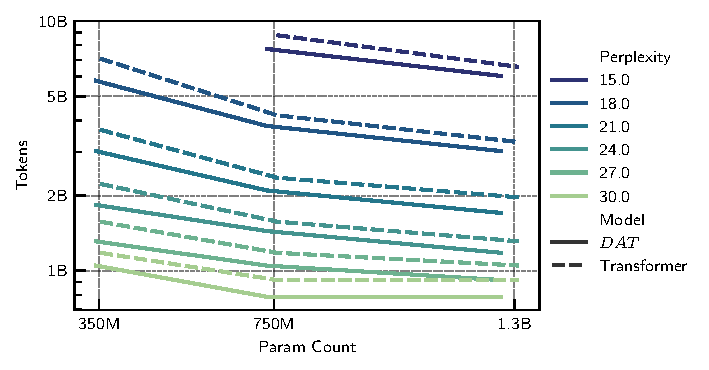
\includegraphics[width=0.7\textwidth]{figs/experiments/fineweb/tokens_vs_param_count.pdf}
    \caption{The \textit{DAT} architecture outperforms standard Transformers in language modeling consistently across model size and data size. This figure depicts the point at which different levels of generalization performance (measured in perplexity) are reached in terms of training tokens for different model sizes. }\label{fig:fineweb_param_data}
\end{figure}
% \begin{table}
%     % \begin{tabular}{@{}l|ccccccc|c@{}}
\begin{tabular}{@{}lcc|cccccc|c@{}}
    \toprule
    Model        & Param count   &$\dmodel$&$\nlayers$& $\nhsa$  & $\nhra$ & $d_r$ & $n_{kv}^{h}$  \\ \midrule\hline
    Transformer  & 353M   & 1024    & 24       & 16       & -        & -     & -           \\
    % \textit{DAT} & 343M   & 1024    & 24       & 8        & 8        & 8     & 4           \\
    % \textit{DAT} & 343M   & 1024    & 24       & 8        & 8        & 32    & 4           \\
    \textit{DAT} & 343M   & 1024    & 24       & 8        & 8        & 64    & 4           \\\midrule
    Transformer  & 757M   & 1536    & 24       & 24       & -        & -     & -           \\
    \textit{DAT} & 734M   & 1536    & 24       & 12       & 12       & 64     & 6          \\\midrule
    Transformer  & 1.31B  & 2048    & 24       & 32       & -        & -     & -           \\
    % \textit{DAT} & 1.27B  & 2048    & 24       & 16       & 16       & 64    & 8           \\
    \textit{DAT} & 1.27B  & 2048    & 24       & 16       & 16       & 128   & 8           \\\bottomrule
    % \textit{DAT} & 1.37B  & 2048    & 24       & 16       & 16       & 64    & -           \\ \bottomrule
\end{tabular}%

% \end{table}

% \begin{minipage}{0.5\linewidth}
%     \centering
%     \resizebox{\linewidth}{!}{
%     % \begin{tabular}{@{}l|ccccccc|c@{}}
\begin{tabular}{@{}lcc|cccccc|c@{}}
    \toprule
    Model        & Param count   &$\dmodel$&$\nlayers$& $\nhsa$  & $\nhra$ & $d_r$ & $n_{kv}^{h}$  \\ \midrule\hline
    Transformer  & 353M   & 1024    & 24       & 16       & -        & -     & -           \\
    % \textit{DAT} & 343M   & 1024    & 24       & 8        & 8        & 8     & 4           \\
    % \textit{DAT} & 343M   & 1024    & 24       & 8        & 8        & 32    & 4           \\
    \textit{DAT} & 343M   & 1024    & 24       & 8        & 8        & 64    & 4           \\\midrule
    Transformer  & 757M   & 1536    & 24       & 24       & -        & -     & -           \\
    \textit{DAT} & 734M   & 1536    & 24       & 12       & 12       & 64     & 6          \\\midrule
    Transformer  & 1.31B  & 2048    & 24       & 32       & -        & -     & -           \\
    % \textit{DAT} & 1.27B  & 2048    & 24       & 16       & 16       & 64    & 8           \\
    \textit{DAT} & 1.27B  & 2048    & 24       & 16       & 16       & 128   & 8           \\\bottomrule
    % \textit{DAT} & 1.37B  & 2048    & 24       & 16       & 16       & 64    & -           \\ \bottomrule
\end{tabular}%

%     }
% \end{minipage}\hfill
% \begin{minipage}{0.5\linewidth}
%     \centering
%     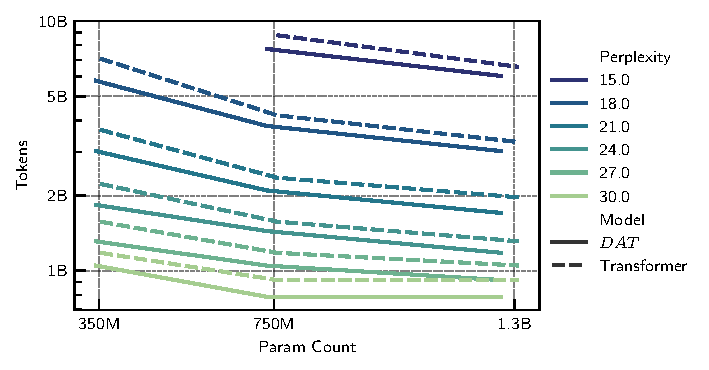
\includegraphics[width=\textwidth]{figs/experiments/fineweb/tokens_vs_param_count.pdf}
%     % \caption{The \textit{DAT} architecture outperforms standard Transformers in language modeling consistently across model size and data size. This figure depicts the point at which different levels of generalization performance (measured in perplexity) are reached in terms of training tokens for different model sizes. }\label{fig:fineweb_param_data}
% \end{minipage}

\Cref{fig:fineweb_param_data} depicts the scaling properties of \textit{DAT}'s language modeling performance with respect to model size and dataset size compared to a standard Transformer. We observe that \textit{DAT} achieves smaller loss with less data across all model scales we tested. This suggests that \textit{DAT}'s relational computational mechanisms confers benefits in language processing.

Beyond performance improvements in language modeling as measured by a drop in perplexity, we also find evidence that relational attention encodes human-interpretable semantic relations. \Cref{fig:datlm_viz} depicts a visualization of the relations $\boldsymbol{r}_{ij}$ learned by a \textit{DAT} language model. We observe that the relations learned by relational attention tend to encode semantic relations, rather than syntactic relations. That is, relational activations $\boldsymbol{r}_{ij} \in \reals^{d_r}$ are high between tokens with related \textit{meanings}. This is in contrast to the attention scores of standard Transformers, where attention heads typically focus on position, syntax, and punctuation~\citep{clark2019doesbertlookat,htut2019attentionheadsberttrack,elhage2021mathematical}, rather than semantic content. We believe that further exploration of this phenomenon from a mechanistic interpretability perspective could offer an exciting avenue for future research.

% \begin{figure}
%     \begin{subfigure}[t]{\textwidth}
%         \scalebox{-1}[-1]{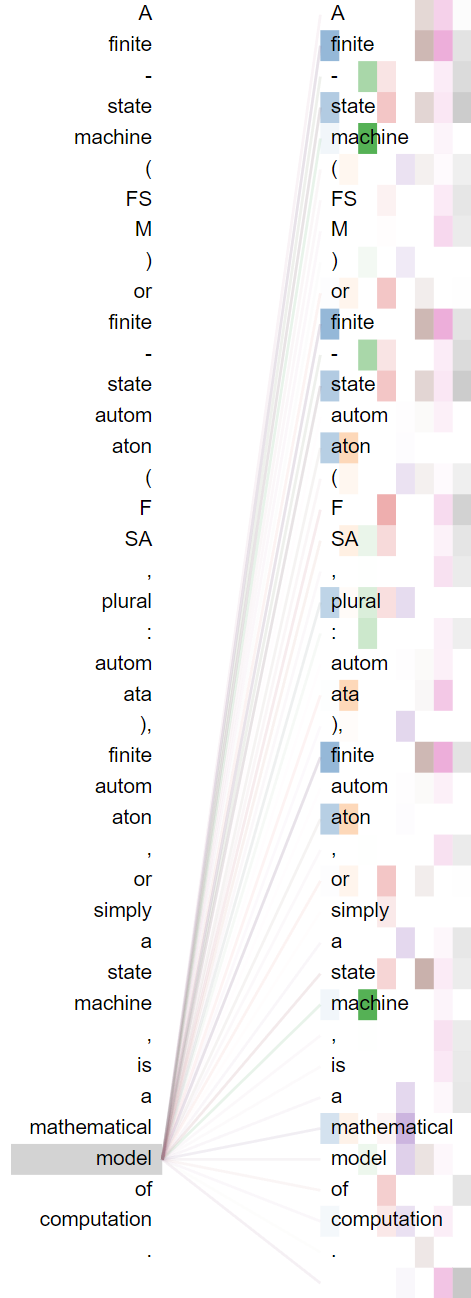
\includegraphics[height=\textwidth, angle=-90]{figs/experiments/fineweb/viz/DAT-343M-viz-L1-allrels-model.png}}
%         % \caption{}\label{fig:}
%     \end{subfigure}
%     \begin{subfigure}[t]{\textwidth}
%         \scalebox{-1}[-1]{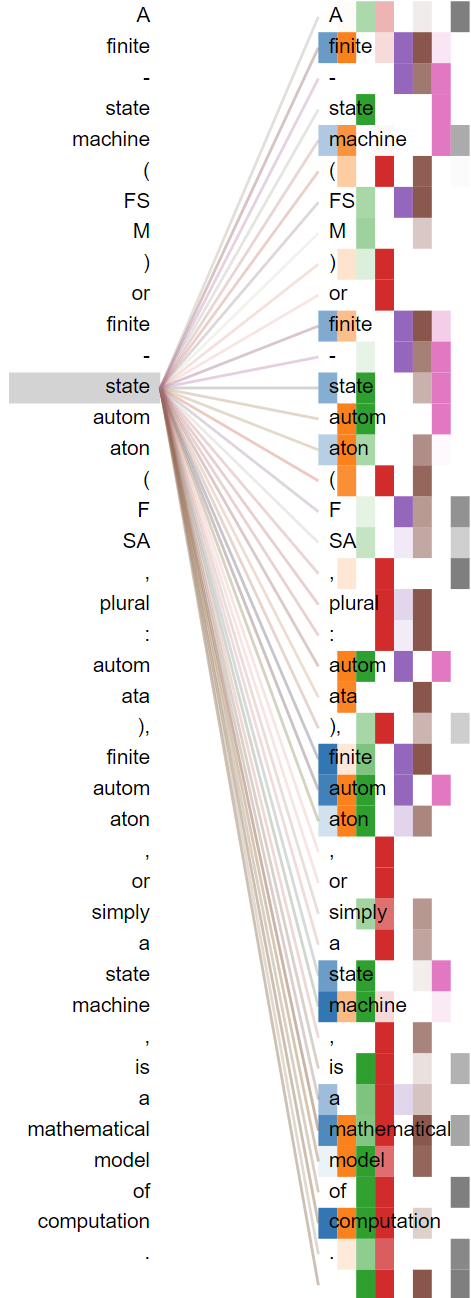
\includegraphics[height=\textwidth, angle=-90]{figs/experiments/fineweb/viz/DAT-343M-viz-L12-allrels-state.png}}
%         % \caption{}\label{fig:}
%     \end{subfigure}
%     \caption{}\label{fig:}
% \end{figure}

\begin{figure}[t]
    \begin{subfigure}[t]{\textwidth}
        \scalebox{-1}[-1]{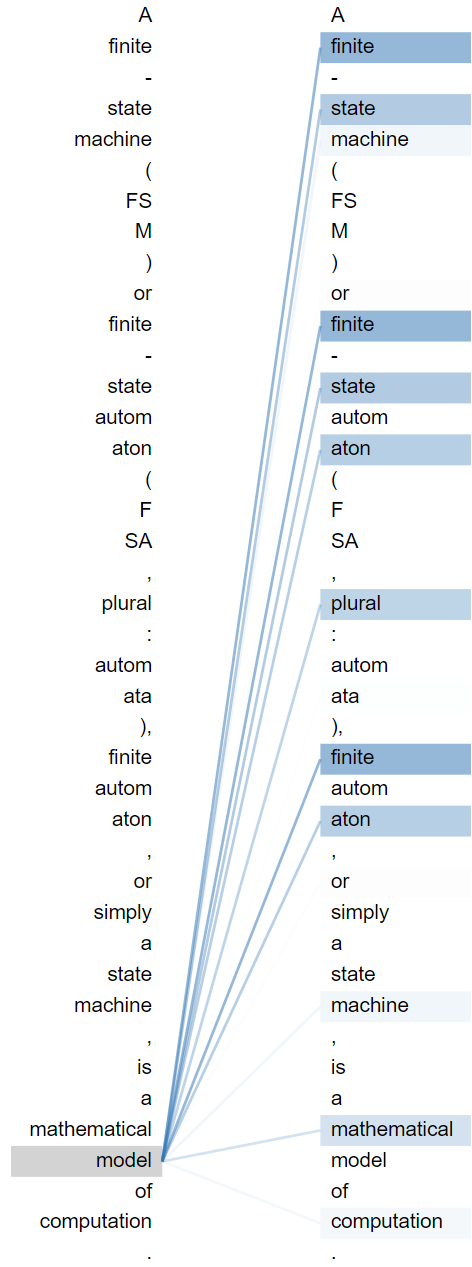
\includegraphics[height=\textwidth, angle=-90]{figs/experiments/fineweb/viz/DAT-343M-viz-L1-rel1-model.png}}
        % \caption{}\label{fig:}
    \end{subfigure}
    \begin{subfigure}[t]{\textwidth}
        \scalebox{-1}[-1]{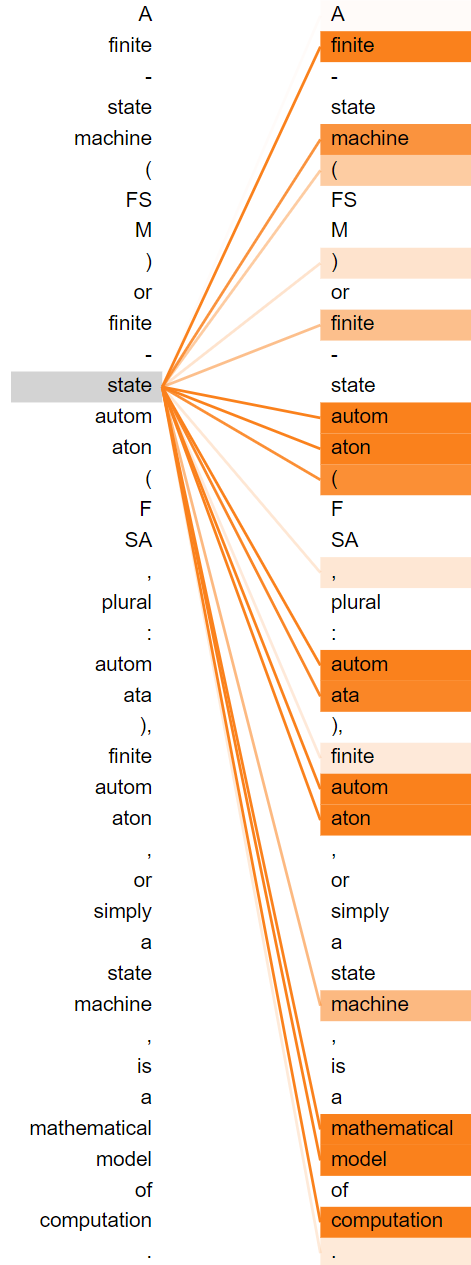
\includegraphics[height=\textwidth, angle=-90]{figs/experiments/fineweb/viz/DAT-343M-viz-L12-rel2-state.png}}
        % \caption{}\label{fig:}
    \end{subfigure}
    \caption{Relational attention in \textit{DAT} language models encodes human-interpretable semantic relations. A visualization of the relations $\boldsymbol{r}_{ij}$ learned by a 24-layer 343M-parameter \textit{DAT} language model. \textbf{Top.} Visualization of one relation dimension in the first layer, focusing on the token \texttt{`model'}, which has high activation with the tokens \texttt{`state'}, \texttt{`machine'}, and \texttt{`mathematical'}. \textbf{Bottom.} Visualization of one relation dimension in the twelfth layer, focusing on the token \texttt{`state'}, which has high activation with the tokens \texttt{`mathematical'}, \texttt{`model'}, and \texttt{`computation'}.}\label{fig:datlm_viz}
\end{figure}

% \begin{figure}[ht]
%     \begin{subfigure}{0.45\textwidth}
%         \centering
%         \captionsetup{width=.9\linewidth}
%         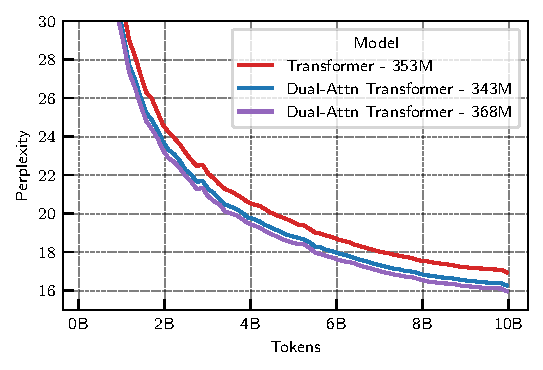
\includegraphics[width=\textwidth]{figs/experiments/fineweb/350M_scale_lm.pdf}
%         \caption{350M parameter scale ($\dmodel = 1024$, $\nlayers = 24$)}
%     \end{subfigure}
%     \begin{subfigure}{0.45\textwidth}
%         \centering
%         \captionsetup{width=.9\linewidth}
%         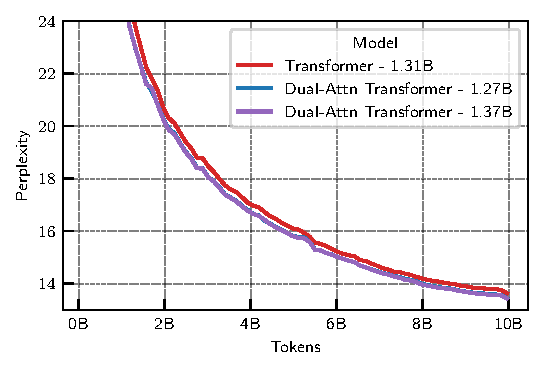
\includegraphics[width=\textwidth]{figs/experiments/fineweb/1_3B_scale_lm.pdf}
%         \caption{1.3B parameter scale ($\dmodel = 2048$, $\nlayers = 24$)}
%     \end{subfigure}
%     \caption{Perplexity curves on language modeling with the fineweb dataset. The $x$-axis indicates the number of tokens and the $y$-axis is the validation perplexity. \textit{DAT} learns faster and achieves smaller perplexity at multiple model size scales.}\label{fig:tiny_stories_val_loss_curves}
% \end{figure}
